% Literature Review
The following literature review will be separated into three sections. The first section describes a general approach to video classification, the second section addresses video classification with respect to advanced driver assistance systems, and the last section considers the existing research in the area of driver attention.

\section{Video Classification}
Video classification in real-world environments find applications in a variety of domains including video surveillance, human action recognition, and intelligent vehicles. Although substantial process has been made in this area, it is still a very challenging problem due to a number of reasons including cluttered backgrounds, occlusions, ambiguity, \emph{etc}. To address these issues, most approaches make strict assumptions about the circumstances under which the video was taken. Additionally, a two-step paradigm is generally followed: (1) compute complex handcrafted features from raw video frames, and (2) learn a classifier based on these obtained features. The main disadvantages with these approaches are most assumptions do not hold true in real-world environments and it is very difficult to know which features are important for a given task.

Deep learning architectures are a class of models that address these problems by learning specific hierarchy features for a given task, and thus, automating the process of feature construction. The follow sections will introduce recent deep learning approaches in video classification.

\subsection{Three-Dimension Convolutional Neural Networks (CNNs)}
One popular deep learning model for understanding image content are convolutional neural networks (CNNs). These models are capable of automatically learning complex features required for vision while yielding state-of-the-art results in image recognition, segmentation, detection, and retrieval. Encouraged by the results in the domain of images, CNN approaches have recently extended into video classification tasks. Compared to still images, video classification tasks require methods to capture additional motion information encoded in adjacent frames. The following section will describe a CNN model that incorporates both spatial and temporal features.

A simple approach to applying CNNs to video classification is to treat each individual frame as a still image and apply a CNN at the individual frame level. Since this approach is applied to two-dimensional images, it does not consider motion information encoded in multiple adjacent frames. To incorporate this information, the work proposed by Ji \emph{et al.}~\cite{3D-CNN:2013} introduces a three-dimensional CNN model applied particularly to action recognition. This model performs three-dimensional convolutions in the convolutional layers of the CNN such that both spatial and temporal dimensions are captured. The full architecture is initialized by generating multiple channels of information from adjacent video frames, \emph{e.g.} gradient and flow information. The model then performs convolution and pooling separately on each information channel. The final feature vector is obtained by combining information from all channels.

In two-dimensional CNNs, convolutions are performed at each convolutional layer to extract features from a local neighborhood on a set of feature maps from the previous layer. An additive bias is then applied and the result is passed through a nonlinear function. Formally, the unit at position $(x,y)$ in the $j^{th}$ feature map in the $i^{th}$ layer, denoted as $v_{ij}^{xy}$, is given by:
\begin{equation}
  v_{ij}^{xy} = tanh\left( b_{ij} + \sum_{m}\sum_{p=0}^{P_i-1}\sum_{q=0}^{Q_i-1}
    w_{ijm}^{pq}v_{(i-1)m}^{(x+p)(y+q)} \right)
\end{equation}
where $tanh(.)$ is the hyperbolic tangent function, $b_{ij}$ is the bias for the feature map, $m$ indexes over the set of feature maps in the $(i-1)^{th}$ layer, $w_{ijk}^{pq}$ is the value at the position $(p,q)$ of the kernel connected to the $k^{th}$ feature map, and $P_i$ and $Q_i$ are the respective height and width of the kernel~\cite{3D-CNN:2013}. The resolution of the feature maps is reduced in the subsampling layers by pooling over a local neighborhood of features. The functionality of these layers is to reduce the spatial size of the feature maps, the number of parameters, and the computation in the network, and thus, controlling overfitting. A CNN architecture is generally constructed by stacking multiple convolutional and subsampling layers in an alternating fashion.

As previously mentioned, these two-dimensional CNNs only compute features from the spatial dimensions. To capture motion information, three-dimensional convolutions are used in the convolutional stages of the CNNs. The 3D convolution is achieved by stacking multiple adjacent frames together. By this construction, the feature maps in the convolutional layer are connected to multiple contiguous frames in the previous layer, thereby capturing motion information. Formally, the value at position $(x,y,z)$ on the $j^{th}$ feature map in the $i^{th}$ layer is given by:
\begin{equation}
  v_{ij}^{xyz} = tanh \left( b_{ij} + \sum_{m}\sum_{p=0}^{P_i-1}\sum_{q=0}^{Q_i-1}\sum_{r=0}^{R_i-1} w_{ijm}^{pqr} v_{(i-1)m}^{(x+p)(y+q)(z+r)} \right)
\end{equation}
where $R_i$ is the size of the 3D kernel along the temporal dimension, $w_{ijm}^{pqr}$ is the $(p,q,r)^{th}$ value of the kernel connected to the $m^{th}$ feature map in the previous layer~\cite{3D-CNN:2013}.

\begin{figure}
  \centering
    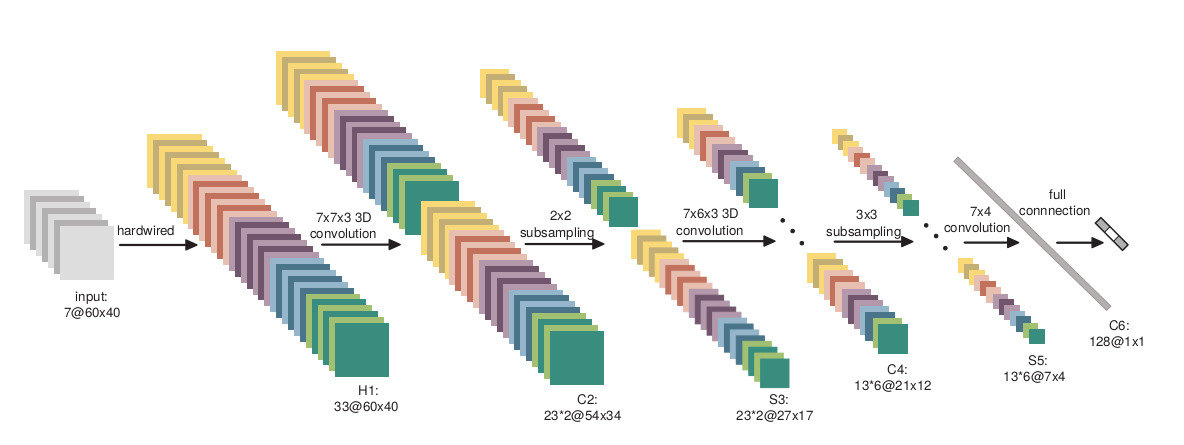
\includegraphics[width=\textwidth]{3d-cnn-architecture}
    \caption{3D CNN architecture. This architecture consists of one hardwired layer, three convolutional layers, two subsampling layers, and a fully connected layer~\cite{3D-CNN:2013}.}
    \label{fig:3D-CNN-architecture}
\end{figure}

The complete 3D-CNN architecture considers several contiguous frames as input. The model is initialized by applying a set of hardwired kernels to the given input sequence to generate multiple channels of information. These five channels consist of the following information: 1) grayscale information where each frame in the input sequence is first converted to a grayscale image, 2) gradient information in both vertical and horizontal directions, and similarly, 3) optical flow information in both vertical and horizontal directions. This hardwired layer is used to encode prior knowledge on the computed features.

Once the five channels of information are computed, the 3D-CNN architecture applies 3D convolutions to each channel respectively, where each 3D convolutional kernel size has an extra temporal dimension $T$. To increase the number of feature maps, two sets of distinct convolutions are applied at each location. These two channels are then passed through alternating pooling and convolutional layers until the last fully-connected layer. The last fully-connected layer incorporates all previous information captured throughout the network, and thus, successfully capturing both spatial and motion information. The full 3D-CNN architecture, along with the respective kernel and feature sizes, is shown in figure~\ref{fig:3D-CNN-architecture}. 

The complete architecture was evaluated on the TRECVID 2008 and KTH datasets~\cite{Schuldt:2004}. The TRECVID dataset consists of 49-hours of video captured at the London Gatwick Airport using five different cameras. The architecture focused on the recognition of three action classes in a one-against-rest manner. Additionally, a simple frame-based 2D-CNN architecture was used in comparison. The average precision and recall for both the 3D and 2D-CNN architectures are as follows: the 3D-CNN received an average precision and recall accuracy of $71.37\%$ and $2.30\%$ respectively, while the 2D-CNN architecture received accuracies of $60.85\%$ and $1.55\%$. This comparison demonstrates the benefits of incorporating motion information in the convolutional layers of the CNN architecture. The KTH dataset consists of six action classes performed by $25$ subjects. Using a similar evaluation process to the TRECVID dataset, the 3D-CNN model was compared to other common action recognition models~\cite{Niebles:2008, Jhuang:2007, Schindler:2008}. The 3D-CNN architecture achieved an overall accuracy of $90.2\%$, demonstrating competitive results to the compared methods with accuracies of $83.3\%$,  $91.7\%$, and $92.7\%$ respectively. 

\subsection{Fusion-Based Convolutional Neural Networks}
Unlike images which can be cropped and rescaled to a fixed size, videos vary widely in temporal extent and cannot be easily processed with a fixed-size architecture. The fusion-based CNN architecture proposed by Karpathy \emph{et al.}~\cite{LargeScaleFusionCNN:2014} offers to treat every video as a bag of short, fixed-sized clips. Since each clip contains several contiguous frames in time, the connectivity of the CNN model is extended in the time domain in order to learn spatio-temporal features.

To learn these spatio-temporal features, three proposed fusion methods are evaluated: late fusion, early fusion, and slow fusion. One difficulty with extending CNN models in the time domain is the difficulty of training grows considerably, \emph{i.e.} the network must now process several frames of the video at a time. To address this issue, the proposed architectures are modified to contain two separate streams of processing: 1) a context stream that learns features on low-resolution frames, and 2) a high-resolution fovea stream that only operates on the middle portion of the frame. The single-frame CNN model along with its extension in time via fusion is described below and demonstrated in figure~\ref{fig:fusion-cnn}.

\begin{figure}
  \centering
    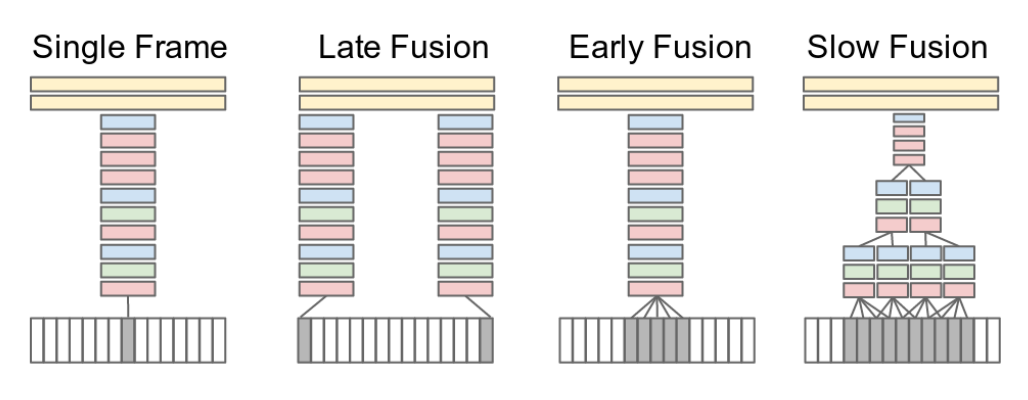
\includegraphics[width=\textwidth]{fusion-cnn}
    \caption{Fusing information over temporal dimensions. Red, green, and blue boxes indicate the convolutional, normalization, and pooling layers, respectively~\cite{LargeScaleFusionCNN:2014}.}
    \label{fig:fusion-cnn}
\end{figure}

\begin{itemize}
  \item The single-frame model is similar to the ImageNet challenge winning model~\cite{Krizhevsky:2012} as it looks at each frame individually and extracts only spatial information as it passes through the CNN model. The final fully-connected layers contain no motion information from the input frames.
  \item The late fusion model places two separate single-frame networks with shared parameters a distance of $n$ frames apart. This model passes spatial information through the two separate single-frame networks and merges both streams in the first fully-connected layer. Using this approach, neither single-frame network alone can detect any motion but the first fully-connected layer can compute global motion characteristics by comparing the outputs of both towers.
  \item The early fusion model extends on the single-frame fusion model as it combines information across an entire window immediately on the pixel level. To incorporate this information, the filters in the first convolutional layer of the single-frame model are extended by $T$ pixels, where $T$ is some temporal extend. This new spatio-temporal information is then passed forward through the complete network. 
  \item The slow fusion model is a balanced mix between the two approaches. This model slowly fuses temporal information throughout the network such that the higher layers receive progressively more global information in both spatial and temporal dimensions. This model is implemented by extending the connectivity of all convolutional layers in time and carrying out temporal convolutions in addition to spatial convolutions to activations.
\end{itemize}

\begin{figure}
  \centering
    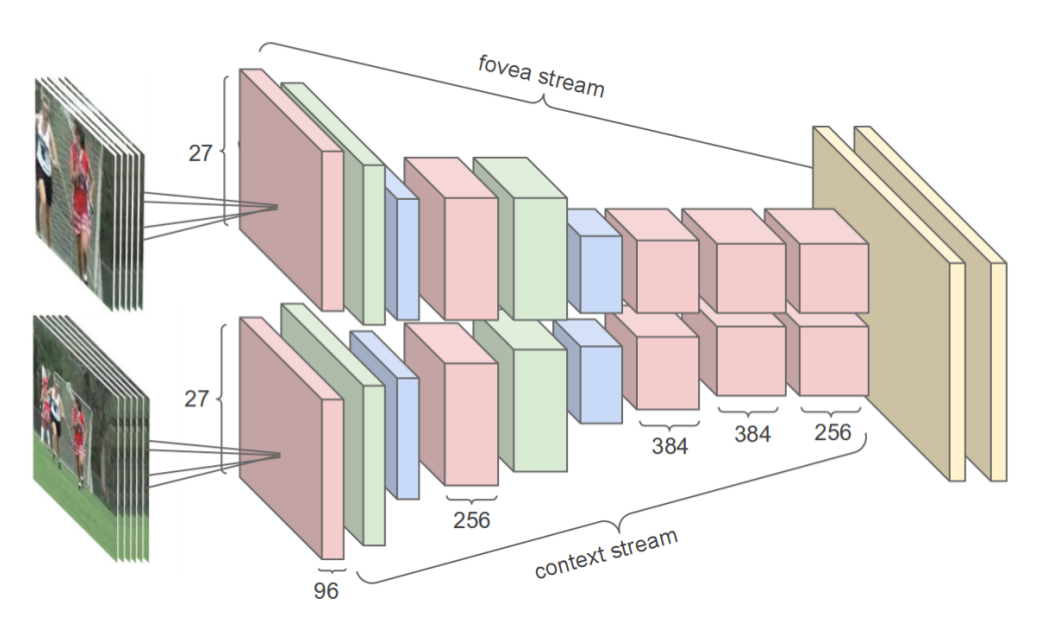
\includegraphics[width=0.6\textwidth]{multireso-cnn}
    \caption{Multi-resolution CNN architecture. Both streams consist of convolution (red), normalization (green), and pooling (blue) layers. The streams converge via two fully-connected layers (yellow)~\cite{LargeScaleFusionCNN:2014}.}
    \label{fig:multireso-cnn}
\end{figure}

To train the fusion-based models takes considerably more time than training the single-frame approach, and thus, a multi-resolution architecture is used. This architecture aims to balance the speed of low-resolution training with the accuracy of high-resolution training. The low-resolution context stream receives the downsampled frames at half the original spatial resolution, while the fovea stream receives the center region at the original resolution. Using the two-stream approach, the total input dimensionality is reduced by half. The complete architecture processes both streams by the same networks described above, with the small adjustment of starting at half the original input resolution. The final activations from both streams are then concatenated and fed into the first fully connected layer of the network. Figure~\ref{fig:multireso-cnn} demonstrates the final CNN architecture.

The proposed architecture was evaluated on the Sports-1M dataset consisting of one-million YouTube videos annotated with $487$ classes~\cite{LargeScaleFusionCNN:2014}. Using this dataset, the hit-1 and hit-5 (correct prediction in top $k$ predictions) accuracies were computed for both the single-frame approach and the early, late, and slow fusion approaches. Table~\ref{tab:fusion-cnn} demonstrate these results. It is evident that incorporating additional motion information via late and slow fusion provides additional insight into the video classification task.

Additional, transfer learning was conducted on the UCF-101 Activity Recognition dataset~\cite{UCF-101}. This dataset consists of $13,320$ videos belonging to $101$ categories. The same slow fusion network that was trained on the Sports-1M dataset was then evaluated on the UCF-101 dataset scoring a hit-1 accuracy of $65.4\%$ when fine-tuning the top three full-connected layers.

\begin{table}[ht]
  \centering
    \begin{tabular}{|c|l|l|}
      \hline
      \textbf{Model} & \textbf{Hit-1} & \textbf{Hit-5}\\
      \hline
      Single-Frame & 59.3\% & 77.7\% \\
      Early Fusion & 57.7\% & 76.8\% \\
      Late Fusion  & 59.3\% & 78.7\% \\
      Slow Fusion  & 60.9\% & 80.2\% \\
      CNN Average (Single+Early+Late+Slow) & 63.9\% & 82.4\% \\
      \hline
    \end{tabular}
    \caption{Accuracies for the correct prediction in the top $k$ predictions on the Sports-1M dataset via fusion-based CNN architectures~\cite{LargeScaleFusionCNN:2014}.}
    \label{tab:fusion-cnn}
\end{table}

\subsubsection{Two-Stream Convolutional Networks}
The previous methods described above attempt to model both spatial and temporal features within the same network. The two-stream approach, proposed by~\cite{TwoStream:2014}, offers a two-stream convolutional neural network architecture that incorporates both spatial and temporal information in separate streams. The spatial stream, in the form of individual frame appearance, carries information about scenes and objects depicted in the video while the temporal stream, in the form of motion across the frames, conveys the movement of the observer (the camera) and the objects~\cite{TwoStream:2014}. The two streams are then combined in the later layers via late fusion. The proposed architecture is related to the two-stream hypothesis in which the human visual cortex contains two pathways: 1) a ventral stream that performs objection recognition, and 2) a dorsal stream that recognizes motion~\cite{SeparateVisPaths:1992}. Additionally, decoupling of the spatial and temporal networks allow the spatial network to improve its training time by pre-training on large amounts of labelled object data.

\begin{figure}
  \centering
    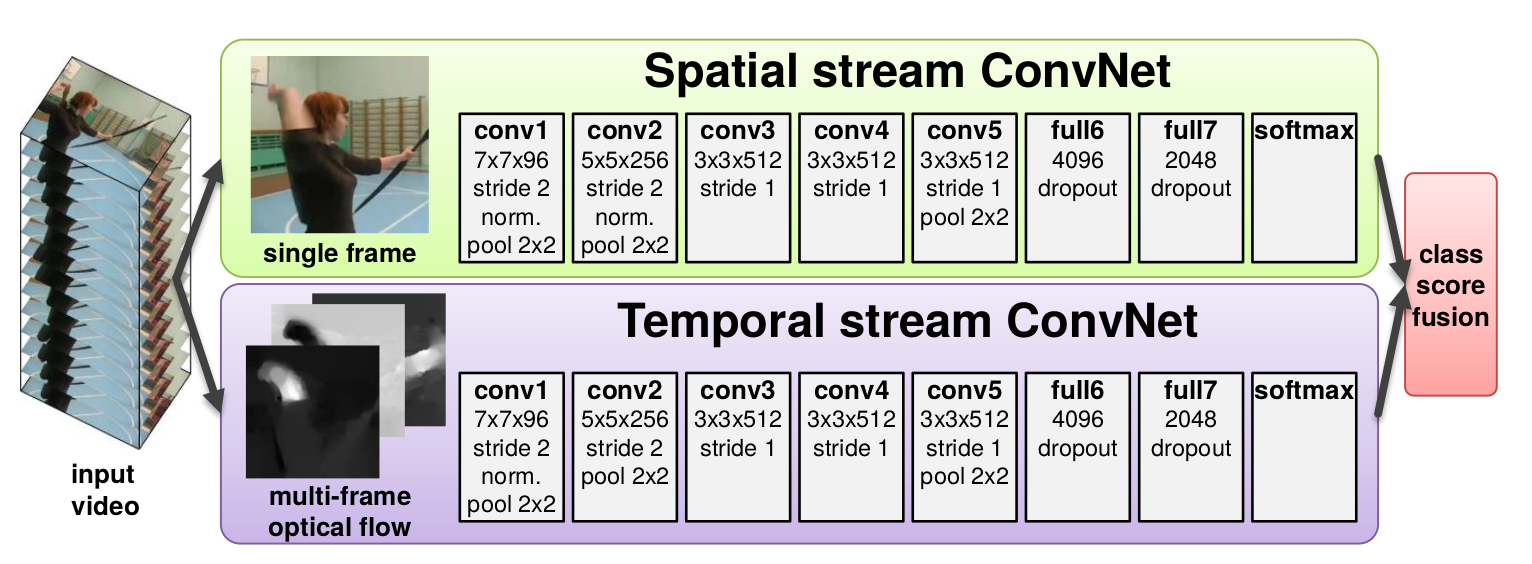
\includegraphics[width=\textwidth]{two-stream}
    \caption{Two-stream architecture for video classification~\cite{TwoStream:2014}.}
    \label{fig:two-stream}
\end{figure}

\begin{figure}
  \centering
    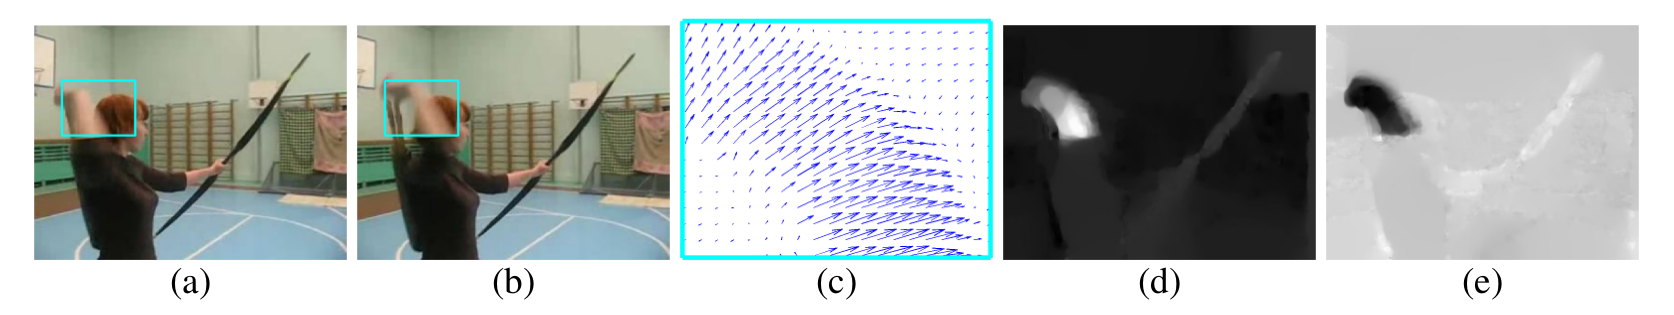
\includegraphics[width=\textwidth]{optflow}
    \caption{Optical Flow. (a)(b): a pair of consecutive frames with the area above the moving hand outlined. (c): a close-up of the dense optical flow in the outlined area. (d)(e): horizontal and vertical component of the displacement field, respectively. Higher intensity corresponds to positive values, while lower intensity to negative values~\cite{TwoStream:2014}.}
    \label{fig:optflow}
\end{figure}

Figure~\ref{fig:two-stream} demonstrates the complete two-stream architecture. As mentioned previously, the spatial ConvNet stream operates on each individual frame in the video, effectively performing action recognition from still images. These appearance features are useful to the complete architecture as some actions are strongly associated to a particular object. The spatial stream in this sense computes the same appearance features as an image classification architecture, and thus, the spatial stream can take advantage of pre-training on a large image classification dataset, \emph{i.e.} the ImageNet dataset~\cite{Krizhevsky:2012}. The temporal stream, which recognizes motion between consecutive frames, operates on optical flow fields. These flow fields explicitly describe the motion between consecutive frames and provides improvement to the training phase as the network does not need to estimate motion implicitly from raw image frames.

The input to the temporal stream is formed by stacking optical flow displacement fields between several consecutive frames. The dense optical flow fields can be seen in figure~\ref{fig:optflow}. The dense optical flow can be represented as set of displacement vector fields $d_t$ between a pair of consecutive frames at $t$ and $t+1$. Using this notation, $d_t(u,v)$ denotes the displacement vector at point $(u,v)$ in frame $t$ that moves to its end location in frame $t+1$. The horizontal and vectors components of the vector field are $d_t^x$ and $d_t^y$ respectively. To represent motion across a sequence of frames, the flow channels of $L$ consecutive frames are stacked, represented by $d_t^{x,y}$, to form a total of $2L$ input channels \cite{TwoStream:2014}. In general, it is beneficial to perform zero-centering of the network input, as it allows the model to better fit the non-linearities. In the case of optical flow, the displacement between a pair of given frames can be dominated by a particular direction, generally caused by camera movement. It is important to compensate for this camera motion, and various methods have attempted to estimate a global displacement vector and subtracting it. The approach used in this architecture is a simple mean subtraction; from each displacement field $d$, the mean vector $(d_x, d_y)$ is subtracted. Once the final compensated inputs are feed into the complete architecture, the output of both CNN streams are a set of softmax scores for each class label. The last layer combines the two sets of softmax scores using a late fusion method based on a multi-class linear support vector machine (SVM) \cite{LinearSVM:2002}.

The complete architecture was evaluated on the UCF-101 dataset~\cite{UCF-101}. Individually, the spatial and temporal streams received a hit-1 accuracy of $72.7\%$ and $81.2\%$ respectively. Using both streams, the final hit-1 accuracy on the UCF-101 dataset was $88.0\%$.


\subsection{Long-Term Recurrent Convolutional Neural Networks}
Recurrent Neural Networks (RNNs) are capable of learning complex temporal dynamics by mapping a given input sequences to a sequence of hidden states, and hidden states to a sequence of outputs via the following recurrence equations:
\begin{align}
  h_t &= g(W_{xh}x_t + W_{hh}h_{t-1} + b_h) \\
  z_t &= g(W_{hz}h_t + b_z)
\end{align}
where $g$ is an element-wise non-linearity, such as a sigmoid or hyperbolic tangent, $x_t$ is the input, $h_t \in \mathbb{R}^N$ is the hidden state with $N$ hidden units, and $y_t$ is the output at time $t$~\cite{LRCN:2015}. Although RNNs have proven successful in various fields, long-term dependencies are difficult to capture due to the well-known vanishing/exploding gradients problem~\cite{LSTM:1997}. This problem results from propagating the gradients down through the many layers of the recurrent network, each corresponding to particular timestep. Long short-term memory units (LSTMs)~\cite{LSTM:1997} provide a solution to this problem by incorporating memory units that allow the network to learn when to forget previous hidden states and when to update hidden states given new information. The equations for the LSTM are as follows:
\begin{align}
  i_t &= \sigma(W_{xi}x_t + W_{hi}h_{t-1} + b_i) \\
  f_t &= \sigma(W_{xf}x_t + W_{hf}h_{t-1} + b_f) \\
  o_t &= \sigma(W_{xo}x_t + W_{ho}h_{t-1} + b_o) \\
  g_t &= \phi(W_{xc}x_t + W_{hc}h_{t-1} + b_c) \\
  c_t &= f_t \odot c_{t-1} + i_t \odot g_t \\
  h_t &= o_t \odot \phi(c_t)
\end{align}
where $\sigma(x) = (1 + e^{-x})^{-1}$ is the sigmoid non-linearity, $\phi(x) = \frac{e^x - e^{-x}}{e^x + e^{-x}}$ is the hyperbolic tangent non-linearity. In addition to the hidden unit $h_t \in \mathbb{R}^N$, the LSTM includes an input gate $i_t \in \mathbb{R}^N$, forget gate $f_t \in \mathbb{R}^N$, output gate $o_t \in \mathbb{R}^N$, input modulation gate $g_t \in \mathbb{R}^N$, and memory cell $c_t \in \mathbb{R}^N$~\cite{LRCN:2015}.

Recently, LSTMs have achieved impressive results in the domains of speech recognition, machine translation, \textit{etc.} Analogous the CNNs, LSTMs are attractive because they allow end-to-end fine-tuning. The advantages of LSTMs for modeling sequential data in vision problems are twofold. First, when integrated with current vision systems, LSTM models are straightforward to fine-tune end-to-end, and secondly, LSTMs are not confined to fixed length inputs or outputs, allowing simple modeling for sequential data of varying lengths, such as text or video. The following sections will demonstrate how LSTMs are used for video classification.


Contrast to the models described above which explore two extrema of perceptual time-series learning, \textit{i.e.} either learning a fully-general time-varying weighting, or applying simple temporal pooling, the proposed Long-term Recurrent Convolutional Network (LRCN)~\cite{LRCN:2015} is ``doubly deep'' in that it can be compositional in both the spatial and temporal ``layers''. Such models have advantages when target concepts are complex and/or training data are limited. Following the same motivation for current deep convolutional models, these models are also deep over the temporal dimension, \textit{i.e.} temporal recurrence of latent variables. The proposed recurrent long-term models are directly connected to modern visual convolutional networks and can be jointly trained to simultaneously learn temporal dynamics and convolutional perceptual representations.


The complete architecture is built on-top of a deep hierarchical visual feature extractor (CNN) with a model that can learn to recognize and synthesize temporal dynamics for tasks involving sequential data. The system works by passing in each visual input, \textit{e.g.} video frame, represented as $v_t$, though a feature transformation $\phi_v(v_t)$ parameterized by $V$ producing a fixed-length vector representation $\phi_t \in \mathbb{R}^d$. Having computed the feature-space representation of the visual input sequence $(\phi_1, \phi_2, \dots, \phi_T)$, the sequence model takes over. The sequence model parameterized by $W$ maps as input $x_t$ and a previous timestep hidden state $h_{t-1}$ to an output $z_t$ and updated hidden state $h_t$. Inference must be ran sequentially, \textit{i.e.} from top to bottom, by computing in order: $h_1 = f_W(x_1, h_0)$, then $h_2 = f_W(x_2, h_1)$, up to $h_T$. The final step is computing the prediction distribution $P(y_t)$ at time-step $t$. To do this, the softmax over outputs $z_t$ of the sequential model, producing a distribution over the space of $C$ possible per-timestep outputs:
\begin{equation}
  P(y_t=c) = \frac{exp(W_{zc}z_{t,c} + b_c)}{\sum_{c' \in C}{exp(W_{zc}z_{t,c'} + b_c)}}
\end{equation}
The visual feature transformation, $\phi$, corresponds to activations in some layer of a deep CNN model. The complete model is shown in figure~\ref{fig:lrcn}.

\begin{figure}
  \centering
    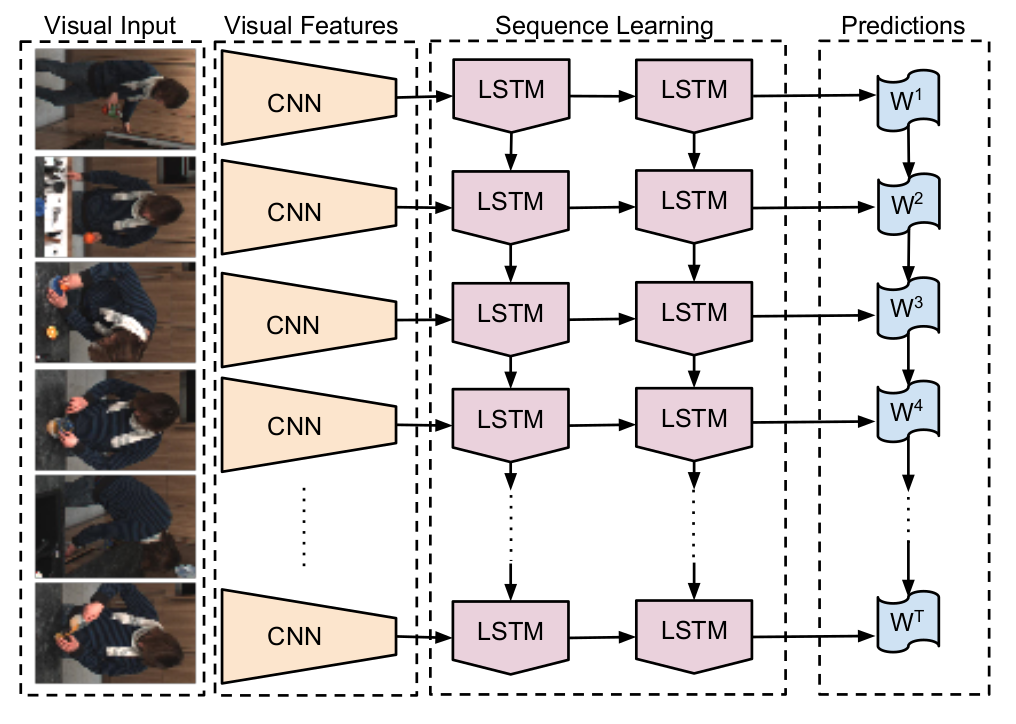
\includegraphics[width=0.6\textwidth]{LRCN}
    \caption{Proposed LRCN architecture. The LRCN processes the variable-length visual inputs (left) with a CNN (middle-left), whose outputs are fed into a stack of recurrent sequence models (LSTMs, middle-right), which finally produce a variable-length prediction (right)~\cite{LRCN:2015}.}
    \label{fig:lrcn}
\end{figure}

The final model takes as input $T$ video frames $(x_1, x_2, \dots, x_T)$ and outputs $T$ labels $(y_1, y_2, \dots, y_T)$. A fusion approached is used to merge per-timestep predictions $(y_1, y_2, \dots, y_T)$ into a single prediction $y$ for the full sequence. The $T$ individual frames are inputs into $T$ convolutional networks which are connected to a single-layer LSTM with $256$ hidden units. The complete model considers both RGB and ``flow-images''. The ``flow-images'' are created by transforming the computed optical flow by centering the $x$ and $y$ values around $128$ and multiplying by a scalar such that the flow values fall between $0$ and $255$. The third channel is created by computing the flow magnitude.

The architecture was evaluated on the UCF-101 dataset~\cite{UCF-101} which consists of 12'000 video categorized into $101$ human action classes. A single-frame baseline architecture was used in comparison to the proposed LRCN network. Table~\ref{tab:lrcn} demonstrates the results. The LRCN model consistently outperforms the baseline model and incorporating RGB and flow helps improve more. This also shows a substantial increase compared to the previous method.

\begin{table}[ht]
  \centering
  \begin{tabular}{|l|c|c|l|c|}
    \hline
    \multirow{2}{*}{} & \multicolumn{2}{c|}{\textbf{Single Input Type}} & \multicolumn{2}{l|}{\textbf{Weighted Average}} \\ \cline{2-5} 
    & \textbf{RGB} & \textbf{Flow} & \textbf{1/2 1/2} & \textbf{1/3 2/3} \\ \hline
    \multicolumn{1}{|c|}{\textbf{Single-Frame}} & 67.70\% & 72.19\% & 75.87\% & 78.84\% \\ \hline
    \multicolumn{1}{|c|}{\textbf{LRCN}} & 68.19\% & 77.46\% & 80.62\% & 82.66\% \\ \hline
  \end{tabular}
  \caption{Comparing single-frame models to LRCN networks for activity recognition on the UCF-101 dataset~\cite{UCF-101}, with both RGB and flow inputs~\cite{LRCN:2015}.}
  \label{tab:lrcn}
\end{table}

\subsubsection{Beyond Short Snippets}


\section{Vehicle Video Classification}

\section{Driver Attention Levels}
